\section{Auswertung einiger Testreihen}\label{sec:Testreihen}
Zur effizienten Untersuchung und Rechnung zahlreicher Beispiele wurden die in Kapitel \ref{sec:algorithmen} aufgezeigten Algorithmen in PARI/GP umgesetzt. (\cite{PARI2018})\\
Alle Beispiele wurden dabei ausschließlich mit dem in Abschnitt \ref{sec:code} gelisteten Programmcode \bzw mithilfe der darin aufgerufenen, nativ in PARI/GP enthaltenen Funktionen gerechnet.
Visualisierungen wurden mit dem Plotting-Framework \emph{pyplot} aus dem \emph{matplotlib 3.1.1}-Paket für Python 3.7 erstellt. Es sei darauf hingewiesen, dass einige der folgenden Grafiken mit logarithmischer, andere mit linearer Skala dargestellt wurden.

\subsection{Methodik}
Zur Testung der genannten Algorithmen wurde die folgende Methodik umgesetzt.
Alle drei Algorithmen durchliefen die Tests zwecks Vergleichbarkeit auf sehr ähnlichen Rechnern mit gleichen Bedingungen, die Laufzeiten sind somit vergleichbar.
Getestet wurde ausgehend von $n \in \N$ mit $3 \leq n \leq 10.000$.
Der Datensatz für ein gewähltes $n$ definiert sich durch die Menge der betrachteten Brüche $M_n = \left\{ \frac{x}{n} \, | \, 1\leq x < n \wedge \text{ggT}(x,n) = 1\right\}$ und enthält neben dem $n$ selbst folgende Eigenschaften, die zugleich den nachgestellten Namen bemkommen:
\begin{itemize}
	\item die durchschnittliche Anzahl der Summanden, \emph{avgTerms(n)}
	\item das Minimum der Anzahl der Summanden, \emph{minTerms(n)}
	\item das Maximum der Anzahl der Summanden, \emph{maxTerms(n)}
	\item das Minimum des jeweils größten Nenners, \emph{minDenom(n)}
	\item das Maximum des jeweils größten Nenners, \emph{maxDenom(n)}.
\end{itemize}
Wird das entsprechende Kriterium nur für einen einzelnen Algorithmus betrachtet, ist dies am Index ersichtlich, der Datenpunkt $n$ der maximalen Anzahl der Terme für den Farey-Folgen-Algorithmus wird beispielsweise durch $maxTerms_{farey}(n)$ angegeben.
Somit entstanden 10.000 Datensätze pro Algorithmus mit jeweils 5 nutzbaren Parametern, insgesamt also 150.000 Datenpunkte, die im Folgenden ausgewertet werden sollen.

\subsection{Anfängliche Probleme und Effizienzsteigerung während der Implementierung}
In den ersten Testläufen traten einige Unannehmlichkeiten auf, da Teile des Codes in der direkten Umsetzung der formalen Beschreibung nicht immer optimal liefen.

\paragraph{Suche nach Nennern im Greedy-Algorithmus}Beispielsweise gab es im ursprünglichen Test des Greedy-Algorithmus den Fall der Zerlegung von $\frac{5}{121}$, dessen Berechnung mittels des Funktionsaufrufs \emph{greedy(5/121)} nach ca. 7 Stunden ohne Ergebnis abgebrochen wurde. Grund hierfür ist das Problem, den größten Stammbruch $\uf{x} \in \Q_+$ zu finden, der kleiner als ein gegebener rationaler Bruch $\frac{p}{q} \in \Q_+$ ist. In der ersten Implementierung wurde dafür in der Folge $(\uf{2}, \uf{3}, \uf{4}, \uf{5},...,\uf{x})$ gesucht, was für große Nenner offensichtlich sehr lange dauert. In einer Optimierung wurde folgende Vorgehensweise umgesetzt, um die Effizienz signifikant zu steigern. Konstruiere die Folge $(\uf{2^1}, \uf{2^2}, ..., \uf{2^k})$ mit $\uf{2^k} > \frac{p}{q} > \uf{2^{k+1}}$. Wähle dann aus dieser Folge mit dem größten Nenner beginnend Elemente aus, die in ihrer Summe kleiner oder gleich $\frac{p}{q}$ sind. Das Ergebnis ist eine Summe von Kehrwerten der gewählten Zweierpotenzen, hier $\uf{x}$ genannt, für die gilt: $\uf{x} \leq \frac{p}{q} < \uf{x-1}$. Somit ist $\uf{x}$ der größte Stammbruch, der kleiner oder gleich $\frac{p}{q}$ ist, wurde aber mit wesentlich weniger Rechenaufwand gefunden.
Dadurch steigerte sich die Effizienz des Greedy-Algorithmus enorm: Das genannte Beispiel $\frac{5}{121}$ wurde in unter einer Millisekunde korrekt berechnet, zahlreiche weitere Beispiele zeigten ähnliche Auswirkungen. Deshalb trägt diese Implementierung auch den Namen \emph{greedy\_fast(fraction)}.

\paragraph{Konstruktion der Farey-Folgen}Ein weiteres Problem stellte die Berechnung der Farey-Folgen dar. Einerseits haben solche Folgen $F_q$ selbst mit mäßig großem $q$ schon sehr viele Elemente, so ist \zB $|F_{280}| = 23.861$; aus den Eigenschaften der Farey-Folgen kann man sehen, dass diese mit steigender Ordnung exponentiell an Größe gewinnen. Andererseits werden die Zähler und Nenner der enthaltenen Brüche mit steigendem $q$ auch größer, was also zusätzlich Speicher belegt und Rechenzeit beansprucht. Nach den ersten Rechnungen wurde schnell klar, dass die vollständige Berechnung der Farey-Folgen zu ineffizient ist und deshalb die Berechnung ausschließlich des relevanten Teils der Farey-Folge, wie es in Beispiel \ref{bsp:Frel} beschrieben ist, umgesetzt wurde. Dies brachte eine signifikante Effizienzsteigerung mit sich.


\subsection{Auswertung der Daten}
Alle nachfolgend aufgeführten Diagramme sind gleichermaßen als Diagramm mit Punktwerten dargestellt, die nicht miteinander verbunden wurden. Abgebildete Linien entstehen durch nahe beieinanderliegende Punkte im Diagramm.


\subsubsection{Laufzeiten}
Die Algorithmen erreichten die folgenden Laufzeiten für die Datensätze $3 \leq n \leq 10.000$:\\
\begin{table}[H]
	\centering
	\begin{tabular}{|l | c c c c|}
		\hline
		\multicolumn{1}{|c|}{\textbf{Algorithmus}} & h & min & sek & ms \\ \hline
		Binär-Algorithmus & & 33 & 22 & 336 \\ \hline
		Greedy-Algorithmus & & 40 &  53 & 499 \\ \hline
		Farey-Folgen-Algorithmus & 62 & 33 & 38 & 136 \\ \hline
	\end{tabular}
	\caption{Laufzeitvergleich der Algorithmen}
	\label{table:LaufzeitVgl}
\end{table}
Die starke Unterlegenheit des Farey-Folgen-Algorithmus ist klar erkenntlich, allerdings nicht mehr wesentlich zu verbessern. Dieses Ergebnis entstand schon mit der in Beispiel \ref{bsp:Frel} beschriebenen Methode, nur die relevante Farey-Folge zu konstruieren, da die Laufzeit mit vollständiger Konstruktion der jeweiligen Farey-Folge für jeden Datensatz $n$ noch höher war. Es lässt sich folgern, dass er damit der laufzeittechnisch schlechteste der drei Algorithmen ist.


\subsubsection{Durchschnittliche Anzahl der Terme}
Eines der wichtigsten Ergebnisse zur realistischen Abschätzung der Algorithmen gegeneinander stellt die durchschnittliche Anzahl der Terme dar, die jeweils durch die Zerlegung entstehen. Abbildung \ref{img:avgTerms} zeigt diese Entwicklung graphisch.
Anhand der Graphen wird das logarithmische Wachstum der Werte erkenntlich. Dabei wird schnell deutlich, dass das Wachstum des Farey-Folgen-Algorithmus bedeutend größer ist als das der anderen beiden Algorithmen. Der Greedy- und der Binär-Algorithmus unterscheiden sich voneinander nicht so stark, offensichtlich schneidet in diesem Kriterium aber der Greedy-Algorithmus mit dem besten Ergebnis ab.
\ifthenelse{\boolean{printGraphics}}{
\begin{figure}[H]
	\caption{Durchschnittliche Anzahl der Terme in Abhängigkeit von $n$}
	\label{img:avgTerms}
	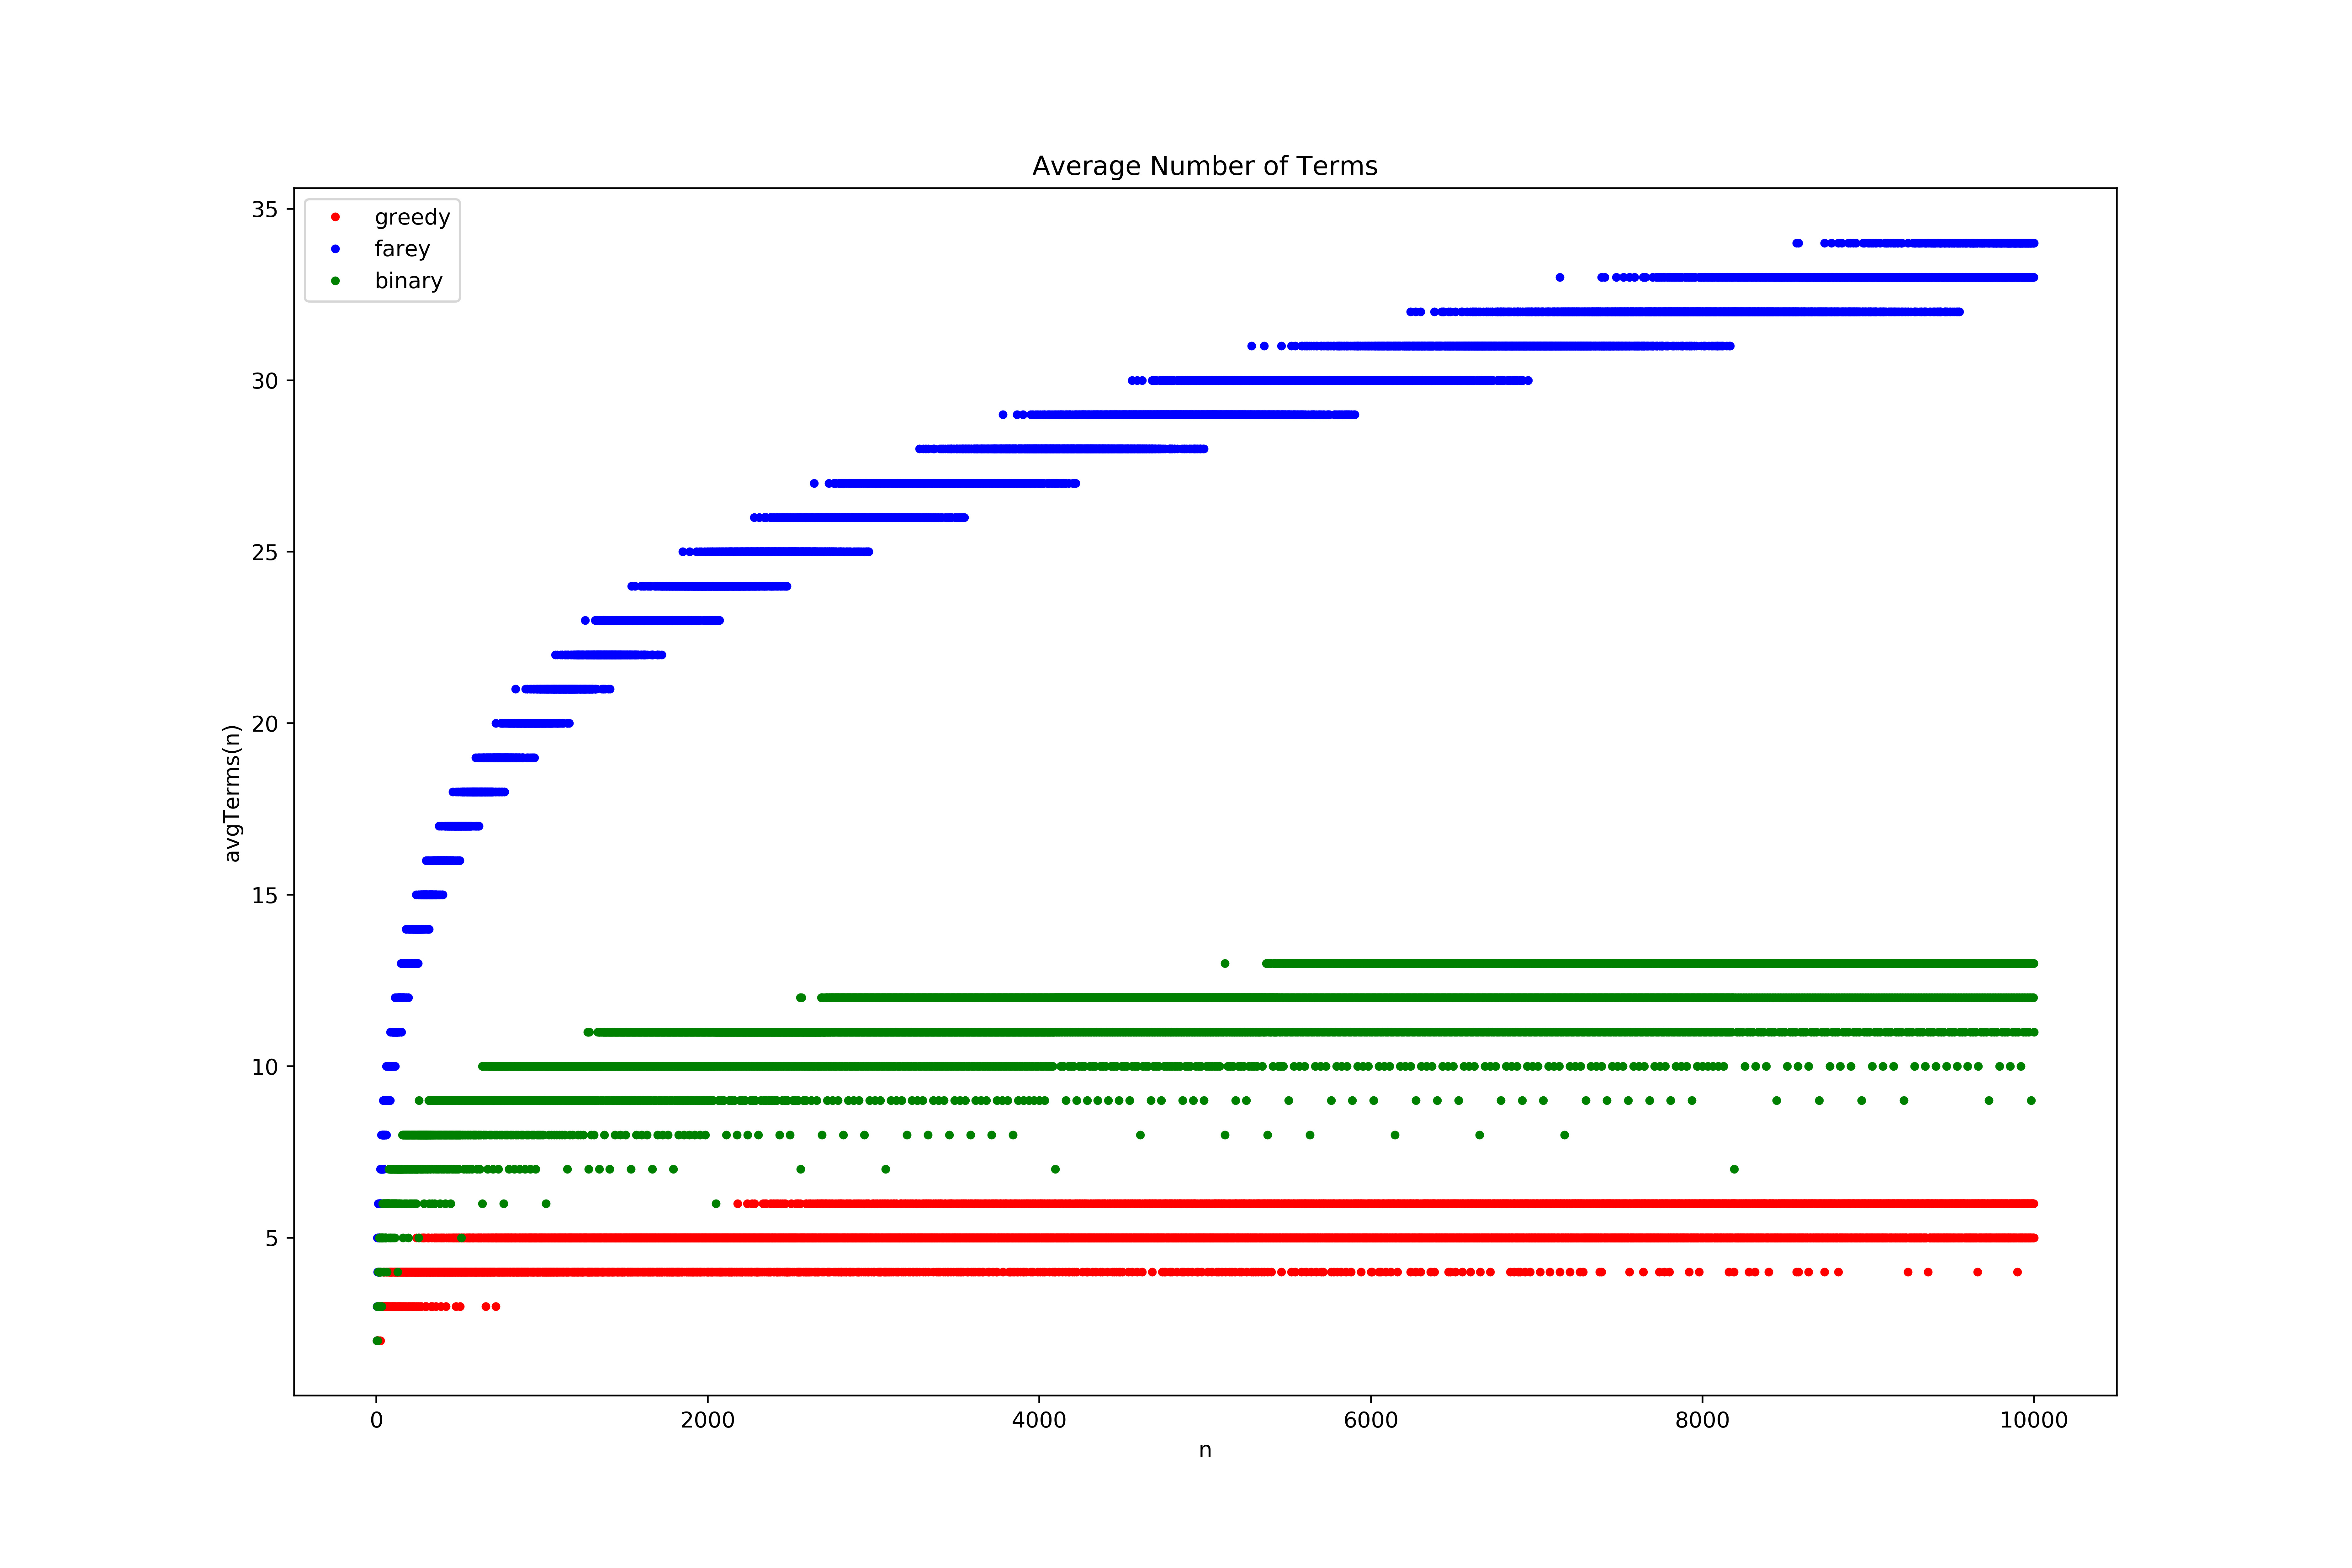
\includegraphics[width=\textwidth]{images/avgTerms.png}
\end{figure}
}{}

\subsubsection{Minimale Anzahl der Terme}
Bezüglich der minimalen Anzahl der produzierten Terme liefert der Greedy-Algorithmus für alle $n$ den gleichen Wert $minTerms_{greedy}(n) = 2$, was jeweils am Ergebnis des Bruchs $\frac{2}{n}$, liegt, welches immer 2 Summanden hat, da der Greedy-Algorithmus jeweils nach der Rechenvorschrift aus Satz \ref{satz:two/n} vorgeht, die wir später noch betrachten werden. Der Farey-Folgen-Algorithmus liefert ständig zwischen $2$ und $3$ alternierende Werte, wobei $n=6$ eine Ausnahme liefert mit $minTerms_{farey}(6) = 5$, da aufgrund der vielen Kürzungen im Datensatz für $n=6$ nur $\frac{5}{6}$ betrachtet wird, welcher in der Farey-Zerlegung 5 Terme benötigt. Beim Binär-Algorithmus erreichen die meisten Tests ein Minimum von 2 Termen pro Datensatz, in ca. $0,7\%$ der Fälle liegt das Minimum jedoch bei 3 Termen. Ein besonderer Zusammenhang zwischen solchen Datensätzen wurde nicht gefunden.

%\ifthenelse{\boolean{printGraphics}}{
%\begin{figure}[H]
%	\label{img:minTerms}
%	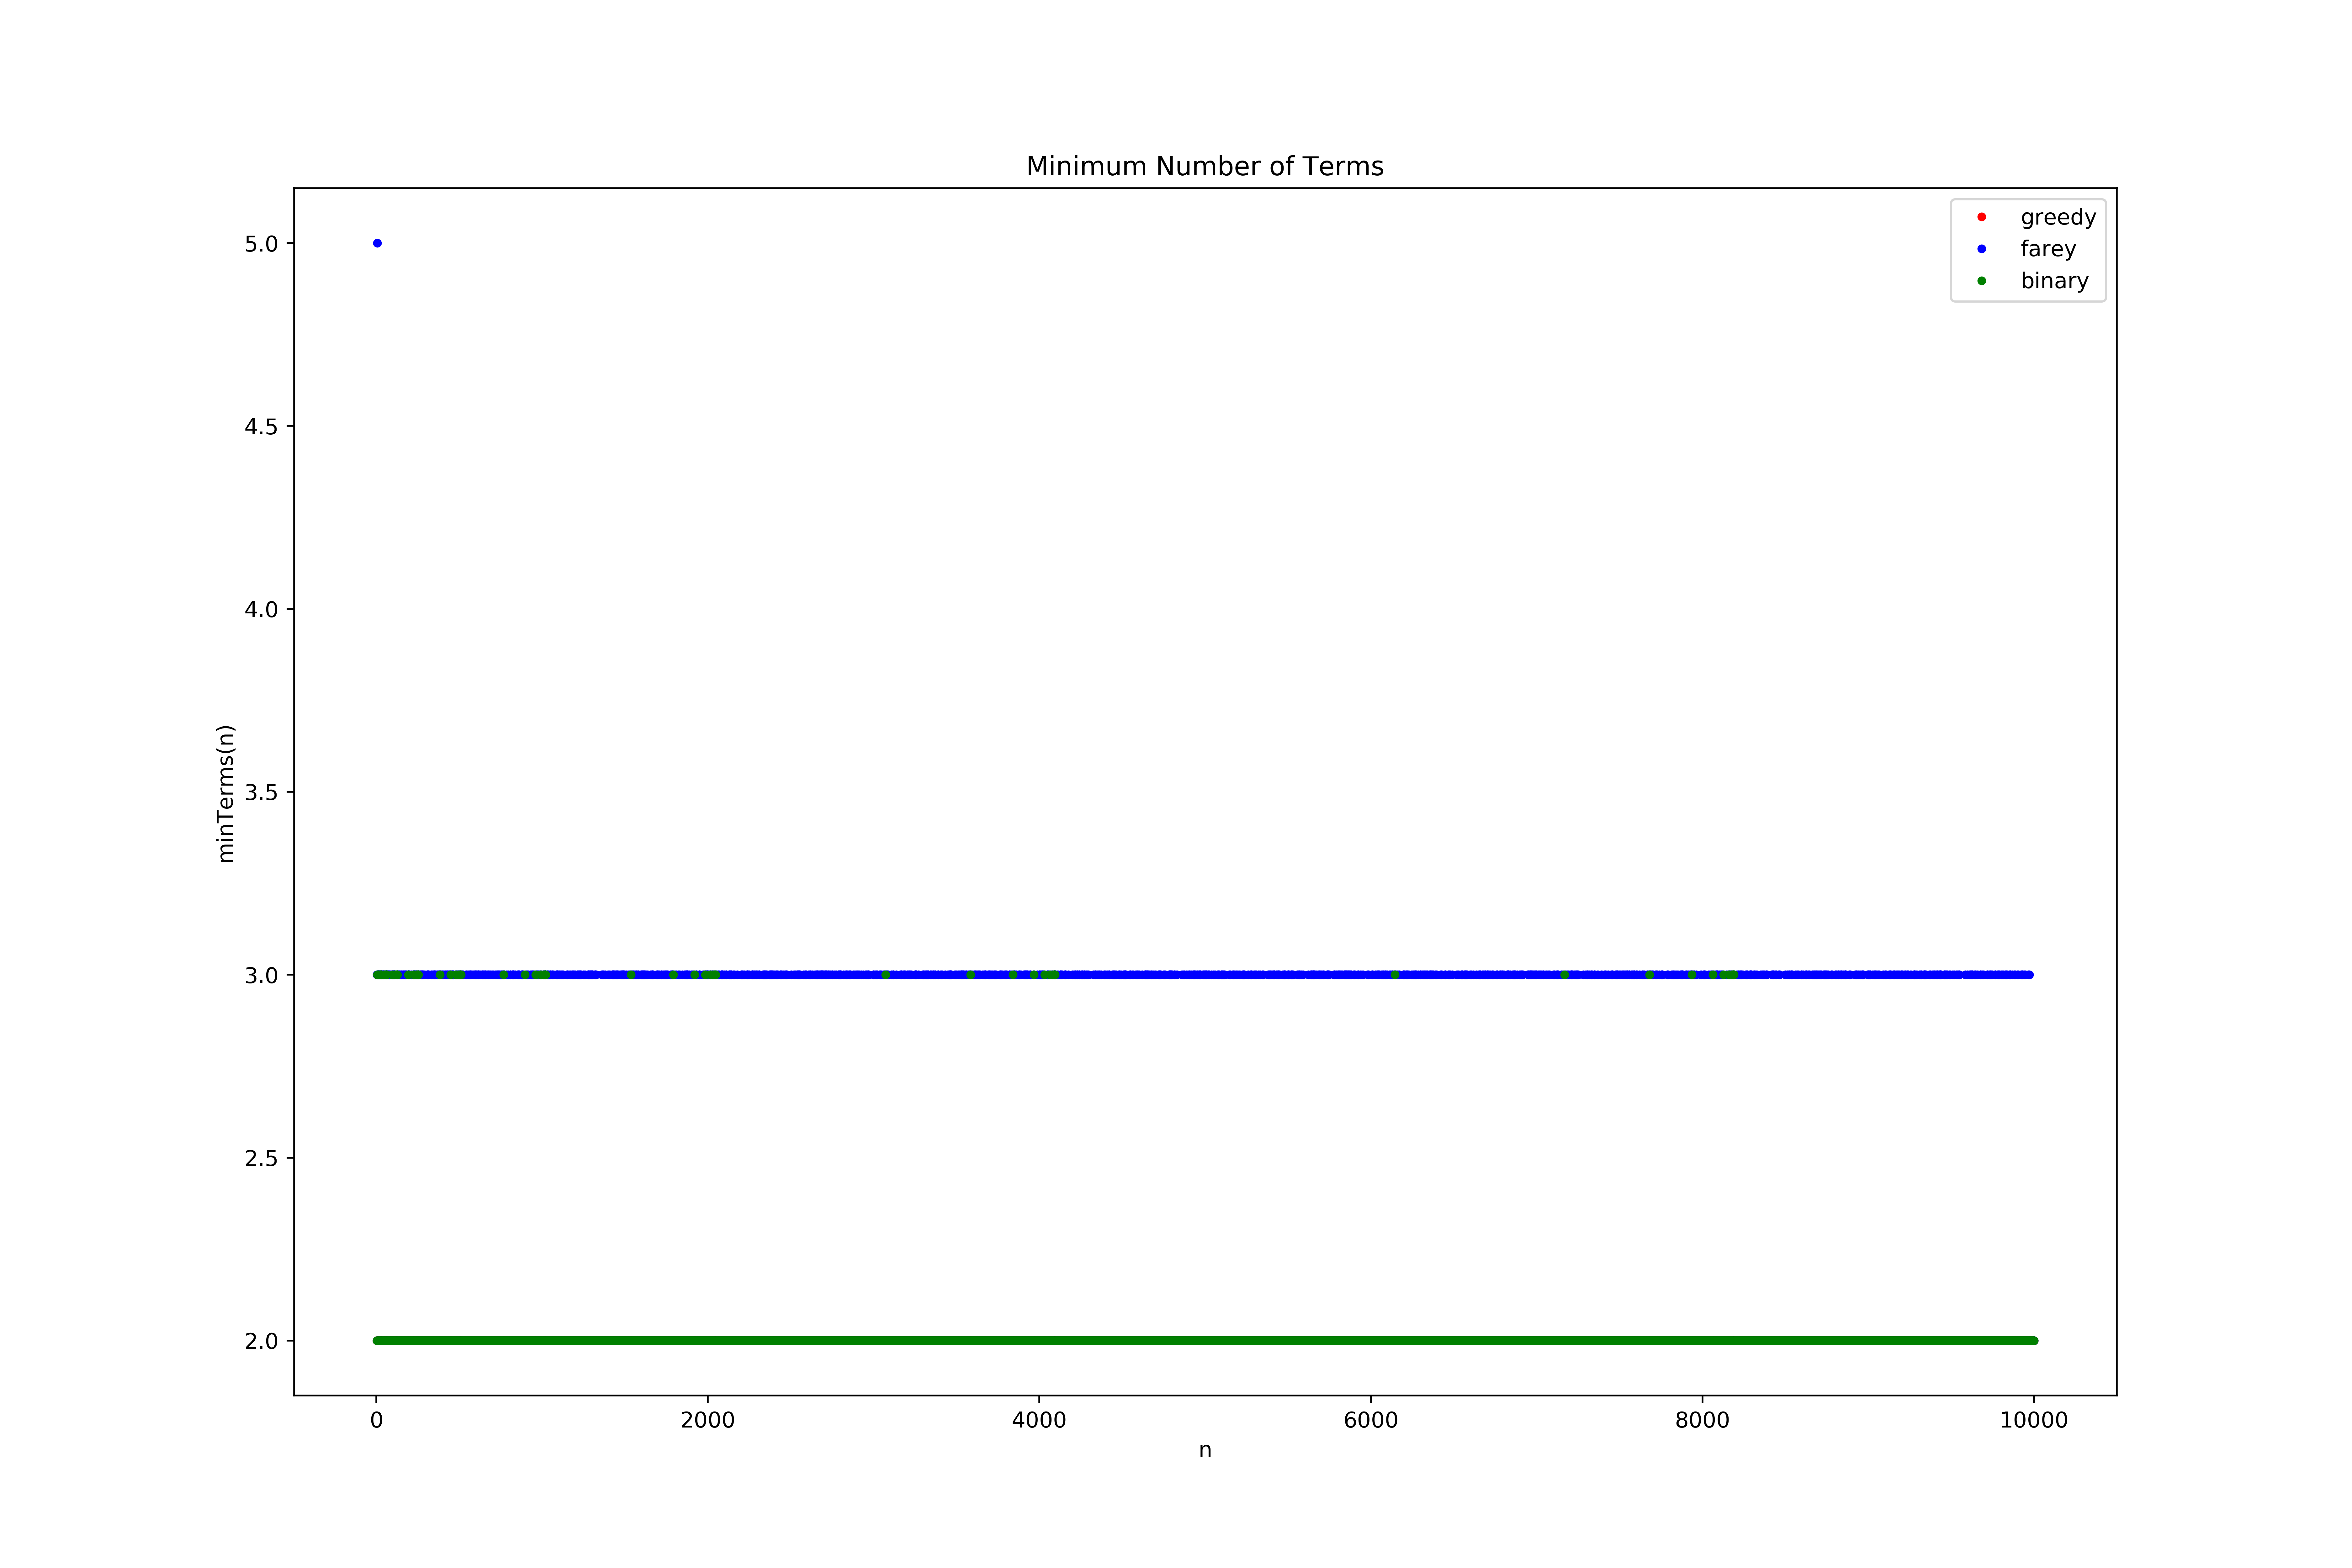
\includegraphics[width=\textwidth]{images/minTerms.png}
%\end{figure}
%}{}


\subsubsection{Maximale Anzahl der Terme}
 Der Greedy-Algorithmus pendelt sich für $3.000 \leq n \leq 10.000$ bei Werten von $7 \leq maxTerms_{greedy}(n) \leq 16$ ein, während der Binäralgorithmus sich im Bereich $2000 \leq n \leq 10.000$ mit Werten von $15 \leq maxTerms_{binary}(n) \leq 22$ mit vernachlässigbar wenig Abweichungen einpendelt. Stiegen die Nenner weiter, wäre das Wachstum nicht beschränkt und würde sich logarithmisch fortsetzen. Für den Farey-Folgen-Algorithmus hingegen gilt ein lineares Wachstum:
$$maxTerms_{farey}(n) = n + 1, \, \forall n$$
für alle getesteten Datensätze. 
\ifthenelse{\boolean{printGraphics}}{
\begin{figure}[H]
	\caption{Maximale Anzahl der Terme im Datensatz für jedes $n$}
	\label{img:maxTerms}
	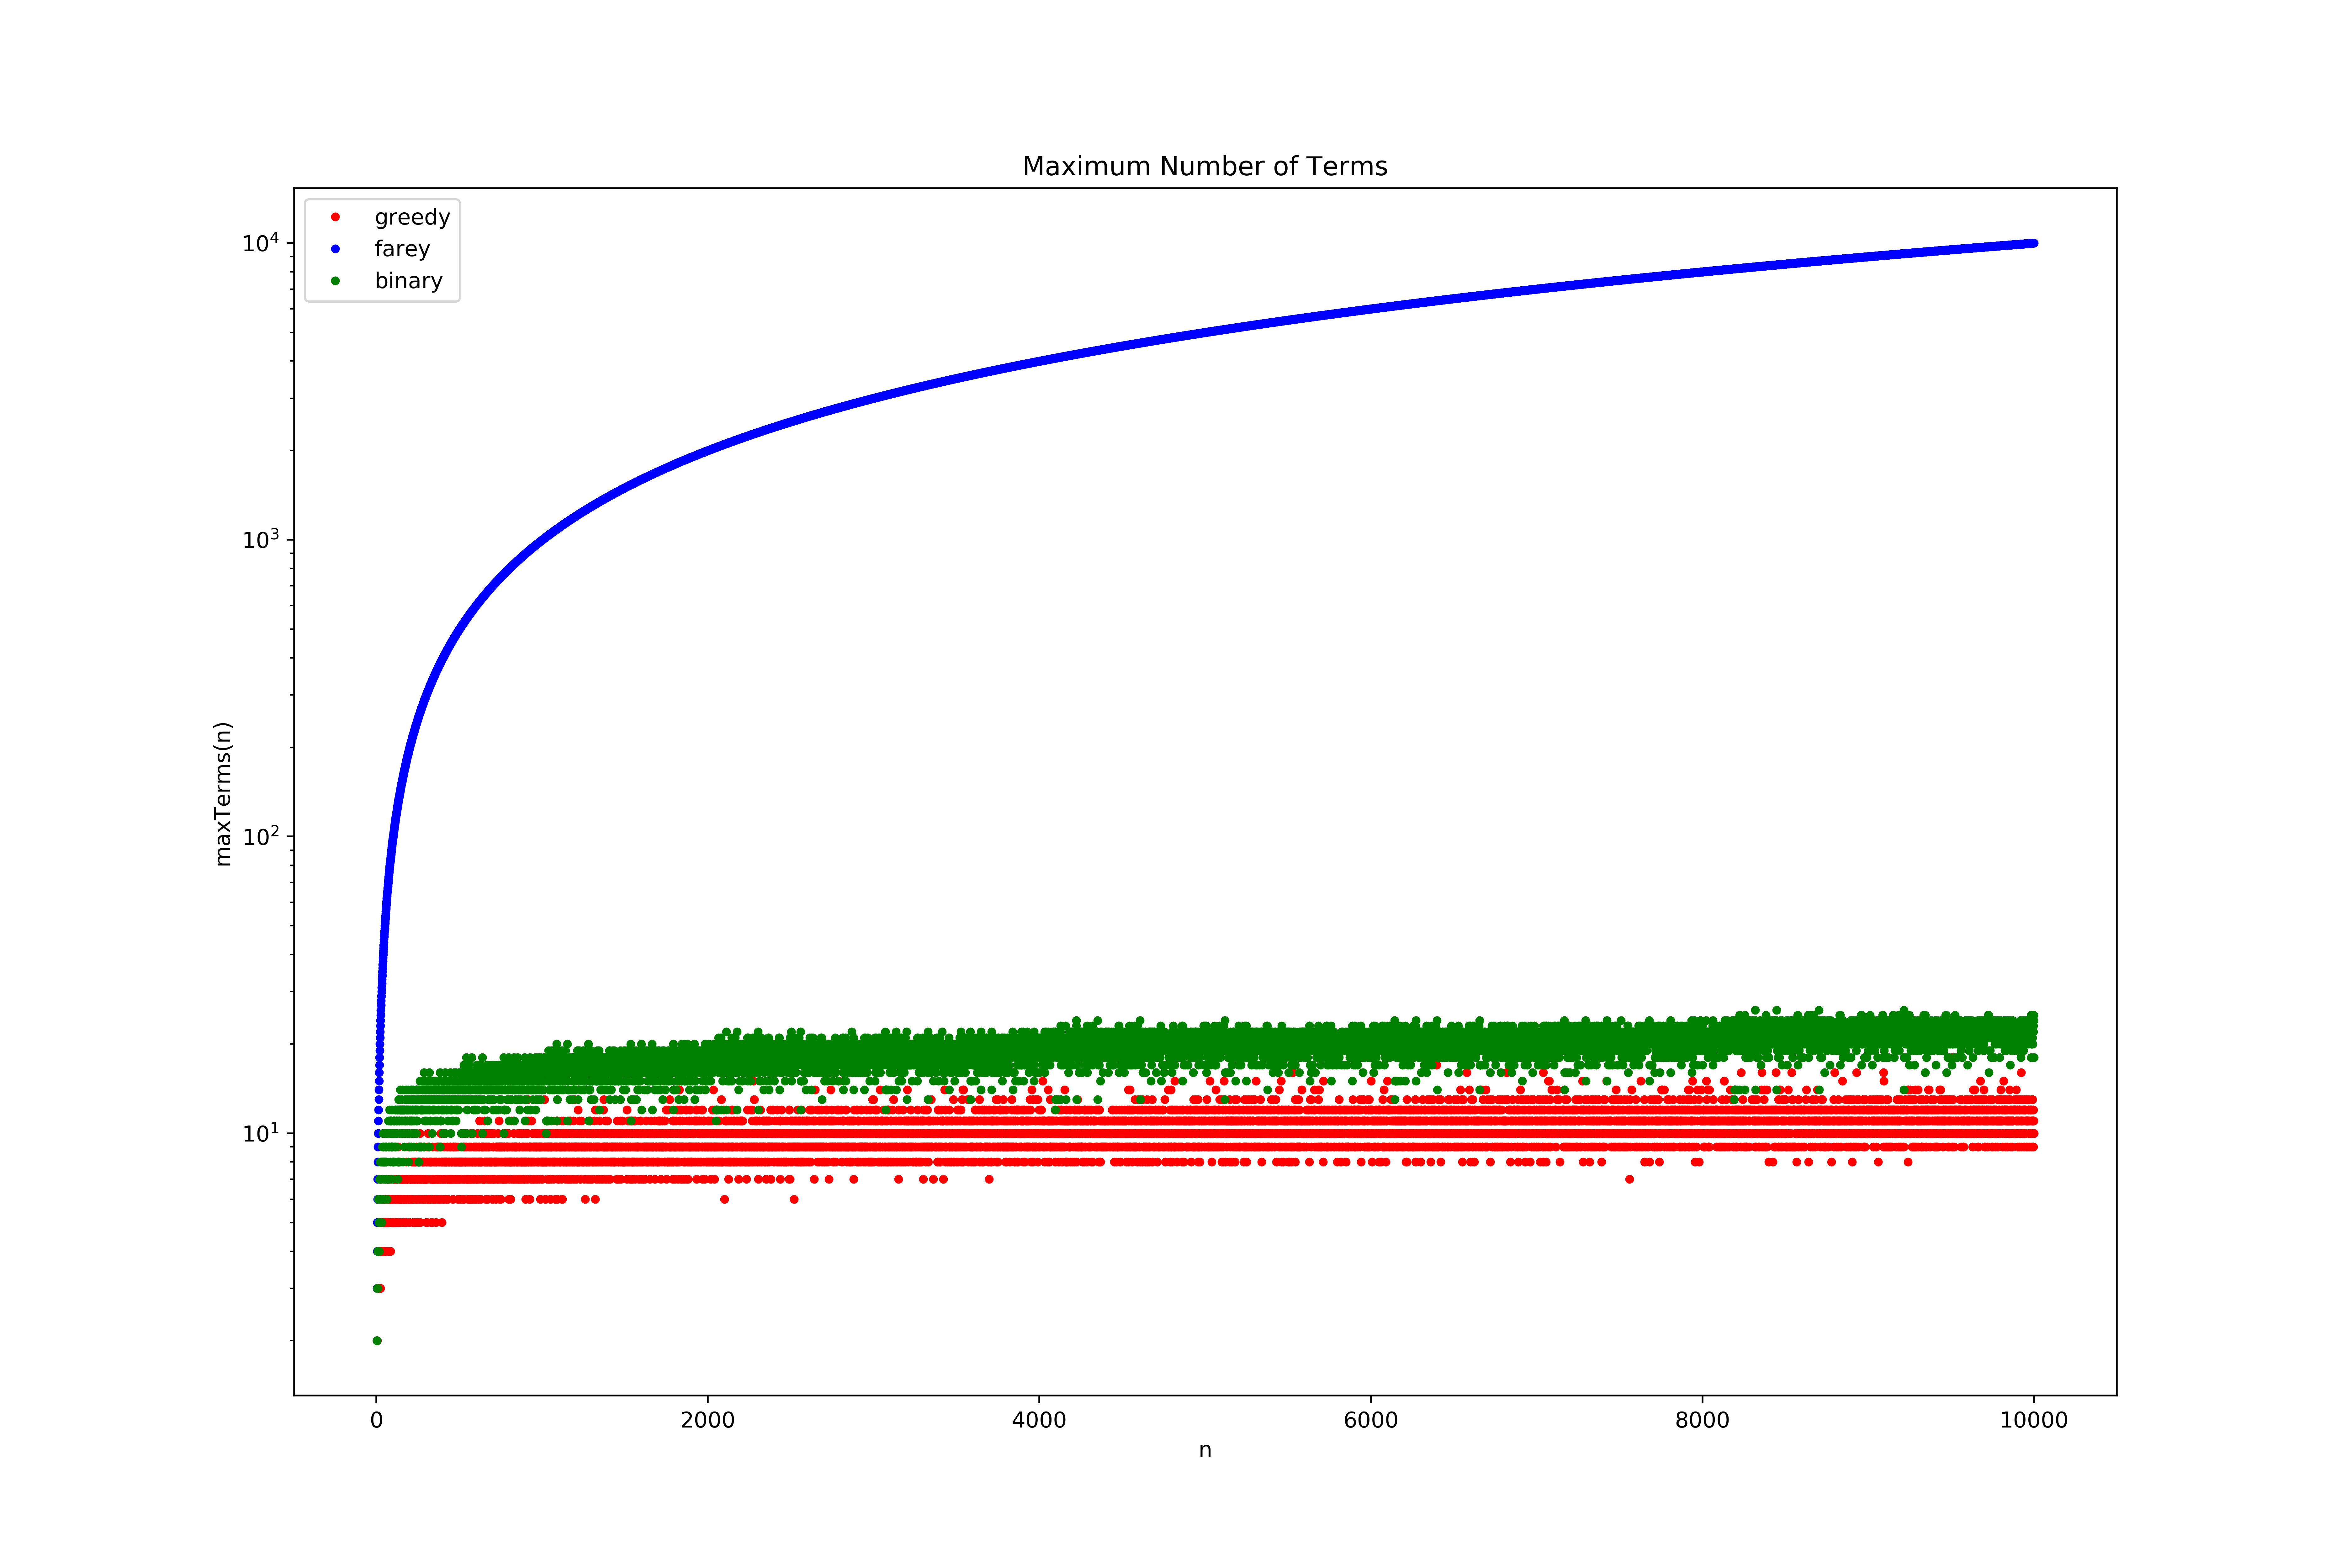
\includegraphics[width=\textwidth]{images/maxTerms.png}
\end{figure}
}{}


\subsubsection{Minimum der größten Nenner}
Sei $u \in \Q$ und bezeichne im Folgenden den Anstieg der linearen Funktion $f(n)=u \cdot n$.\\
Bezüglich des Minimums der größten Nenner zeigen alle Algorithmen klares lineares Wachstum, allerdings in sehr unterschiedlichen Ausprägungen.\\ 
Die Datenpunkte für den Binäralgorithmus ergeben zwei Geraden, eine für alle Werte, bei denen $n$ Zweierpotenz ist, und eine für alle anderen Werte. Das liegt am Sonderfall 2 aus Algorithmus \ref{algo:binary}, der Brüche mit Nennern, die Zweierpotenzen sind, gesondert behandelt und dadurch kleinere Nenner in der Zerlegung produziert. Das lineare Wachstum der beiden Geraden entsteht durch das wachsende $q$ in der Gleichung $\frac{p}{q} = \frac{s}{N_k} + \frac{r}{qN_k}$. Die Gerade der Zweierpotenzen wächst dabei mit Anstieg $u = 1$, die der nicht-Zweierpotenzen mit Anstieg $u=2$. Eine genauere Betrachtung hierzu findet sich im Abschnitt \ref{subsubsec:ZsmHangBinary}\\
Der Greedy-Algorithmus, dessen Werte bzgl. dieses Kriteriums unterhalb und zum Teil auf denen des Binäralgorithmus liegen, zeigt hingegen mehr als zwei Geraden auf, also entwickeln sich bestimmte Folgen innerhalb der Testreihe dieses Algorithmus gleich, die Folgen sind aber in ihrer Entwicklung voneinander unterscheidbar. Die sich ergebenden Geraden haben einen Anstieg $u \in \left\{ 2, 1, \uf{2}, \uf{4}, ... \right\}$, einige Werte liegen aber auch zwischen diesen Geraden. Genaue Gründe hierfür konnten nicht gefunden werden.\\
Ähnliches zeigt sich beim Farey-Folgen-Algorithmus, für den sich 5 Geraden ergeben, allerdings wird hier die Anzahl der Datenpunkte, die jeweils eine Gerade ergeben, mit wachsendem Anstieg immer weniger. Der Anstieg der Geraden ist dabei immer eine Primzahl, die unterste Datenreihe liegt auf der Funktion $f(x)=2x$, die oberste auf der Funktion $f(x) = 13x$. Eine genauere Untersuchung zeigte, dass für jedes fest gewählte $n$ $minDenom_{farey}(n)$ nur durch genau einen Zähler im Datensatz definiert wird. Die Punkte auf der Funktion $f(x) = 13x$ sind beispielsweise durch die Brüche $\frac{1777}{2310}, \frac{1777}{4620}, \frac{6397}{6930} \text{ und } \frac{6397}{9240}$ entstanden. Die scheinbare Logik dahinter wird bereits durch die darunterliegende Gerade $f(x)=11x$ entkräftet, dort tauchen nur die ersten beiden Brüche $\frac{191}{210} \text{ und } \frac{191}{420}$ mit gleichem Zähler zweier aufeinanderfolgender Datenpunkte auf. Allerdings wiederholen sich einige Zähler mehrfach mit unterschiedlichen Nennern, jedoch ohne jegliches erkennbare Muster. Für die Datenpunkte dieser zweithöchsten Gerade sind zudem die Zähler in etwa gleich oft Primzahlen wie nicht Primzahlen. Die Anzahl der Datenpunkte, die auf einer der Geraden liegen, steigt mit sinkendem Anstieg etwa quadratisch.
\ifthenelse{\boolean{printGraphics}}{
\begin{figure}[H]
	\caption{Minimum des größten Nenners im Datensatz für jedes $n$}
	\label{img:minDenom}
	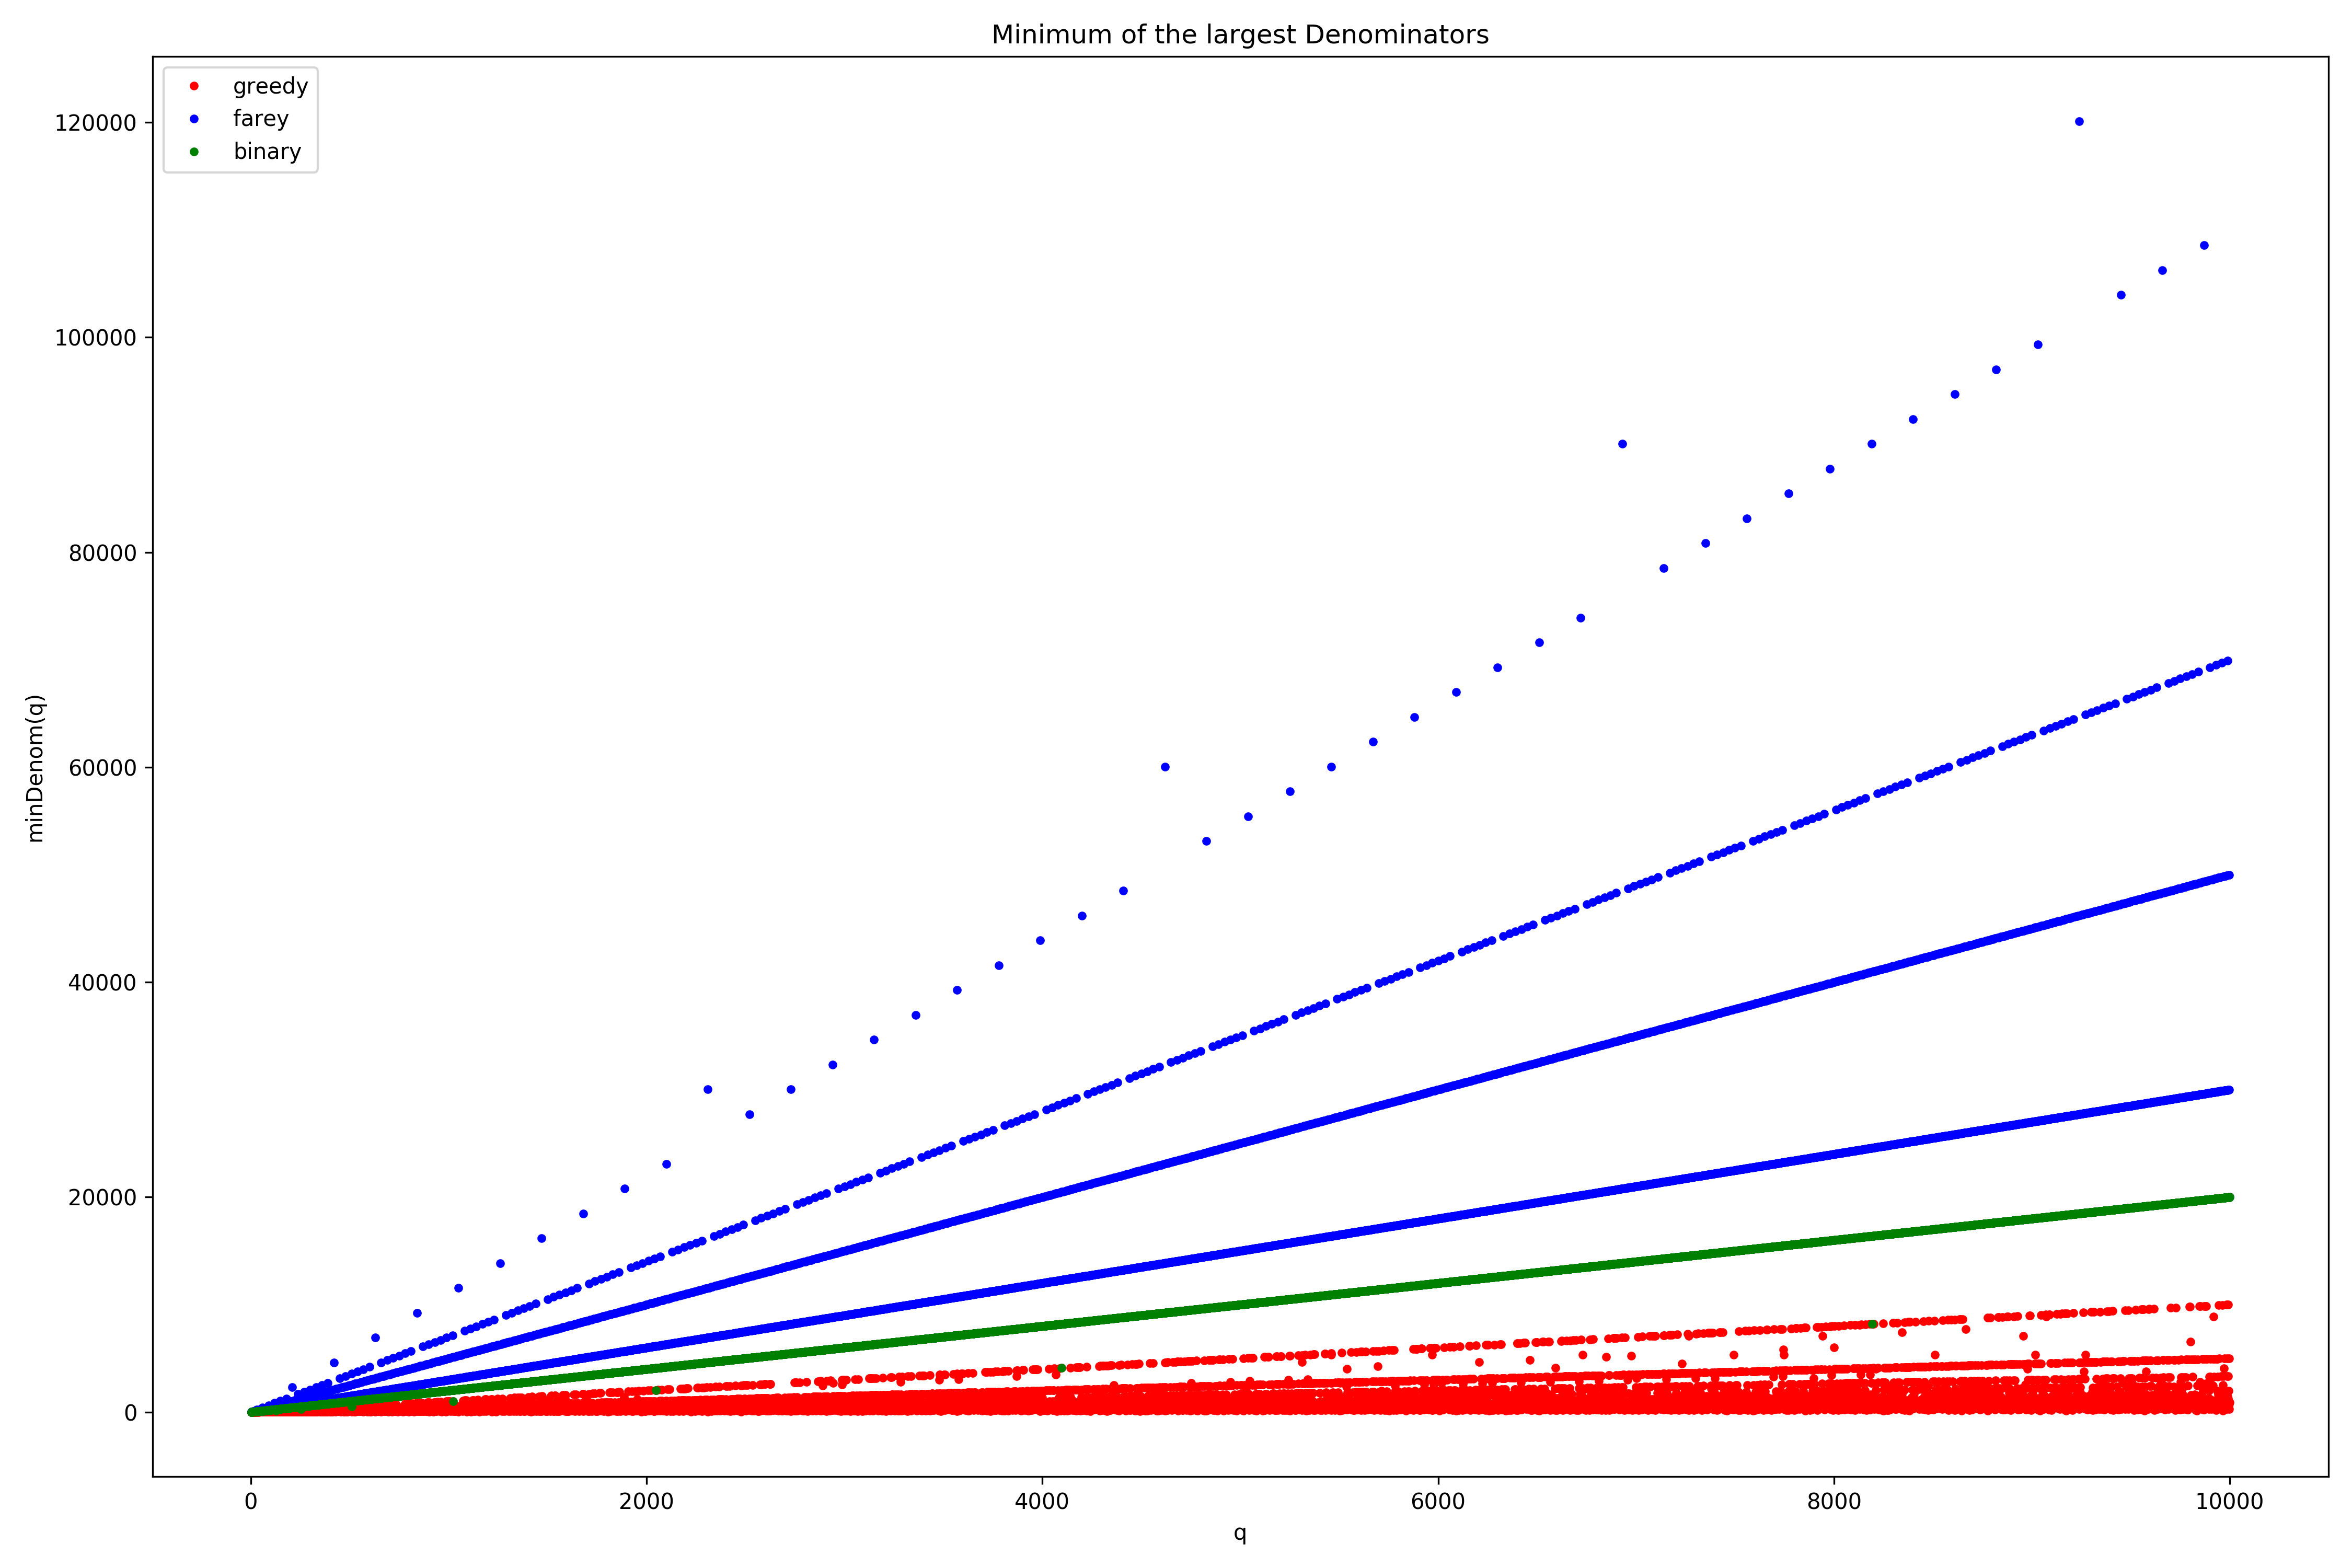
\includegraphics[width=\textwidth]{images/minDenom.png}
\end{figure}
}{}


\subsubsection{Maximum der größten Nenner}
Dieses Kriterium ist jenes, in welchem sich die Algorithmen wohl am stärksten voneinander unterscheiden. Während sich die Werte von Binär- und Farey-Folgen-Algorithmus unter $10^{19}$ halten, streuen sich die Werte des Greedy-Algorithmus von $maxDenom_{greed}(3) = 2$ bis zu einem Maximum von $maxDenom_{greedy}(4967) \approx 7,3378 \times 10^{225.516}$ ohne jegliche erkennbare Regelmäßigkeit. In Abbildung \ref{img:maxDenom} musste auf die Darstellung der 4991 größten Werte des Greedy-Algorithmus verzichtet werden, da diese Werte größer als $10^{250}$ und somit für die Verarbeitung mit \emph{pyplot} zu groß waren.\\
Das Wachstumsverhalten des Binäralgorithmus scheint hier besonders interessant, da sich mehrere Geraden ergeben, die zudem ein sprunghaftes Verhalten aufweisen. Das liegt daran, dass sich der größte Nenner im Binäralgorithmus aus dem Produkt $qN_k$ ergibt, wobei das im Diagramm beschriebene $n=q$ ist. Das $N_k$ ist immer die nächstgrößere Zweierpotenz von $q$, falls $q$ nicht selbst schon eine solche ist. Daher springen die Werte immer bei $q$, falls $q$ Zweierpotenz ist. Das stetig steigende $q$ sorgt zudem für das lineare Wachstum der Geraden, den Anstieg bestimmt $N_k$.\\
Der Farey-Folgen-Algorithmus zeigt für dieses Kriterium ein quadratisches Wachstum auf.

\ifthenelse{\boolean{printGraphics}}{
	\begin{figure}[H]
		\caption{Maximum der größten Nenner pro Datensatz, links: mit Graph für den Greedy-Algorithmus, rechts: ohne selbigen}
		\label{img:maxDenom}
		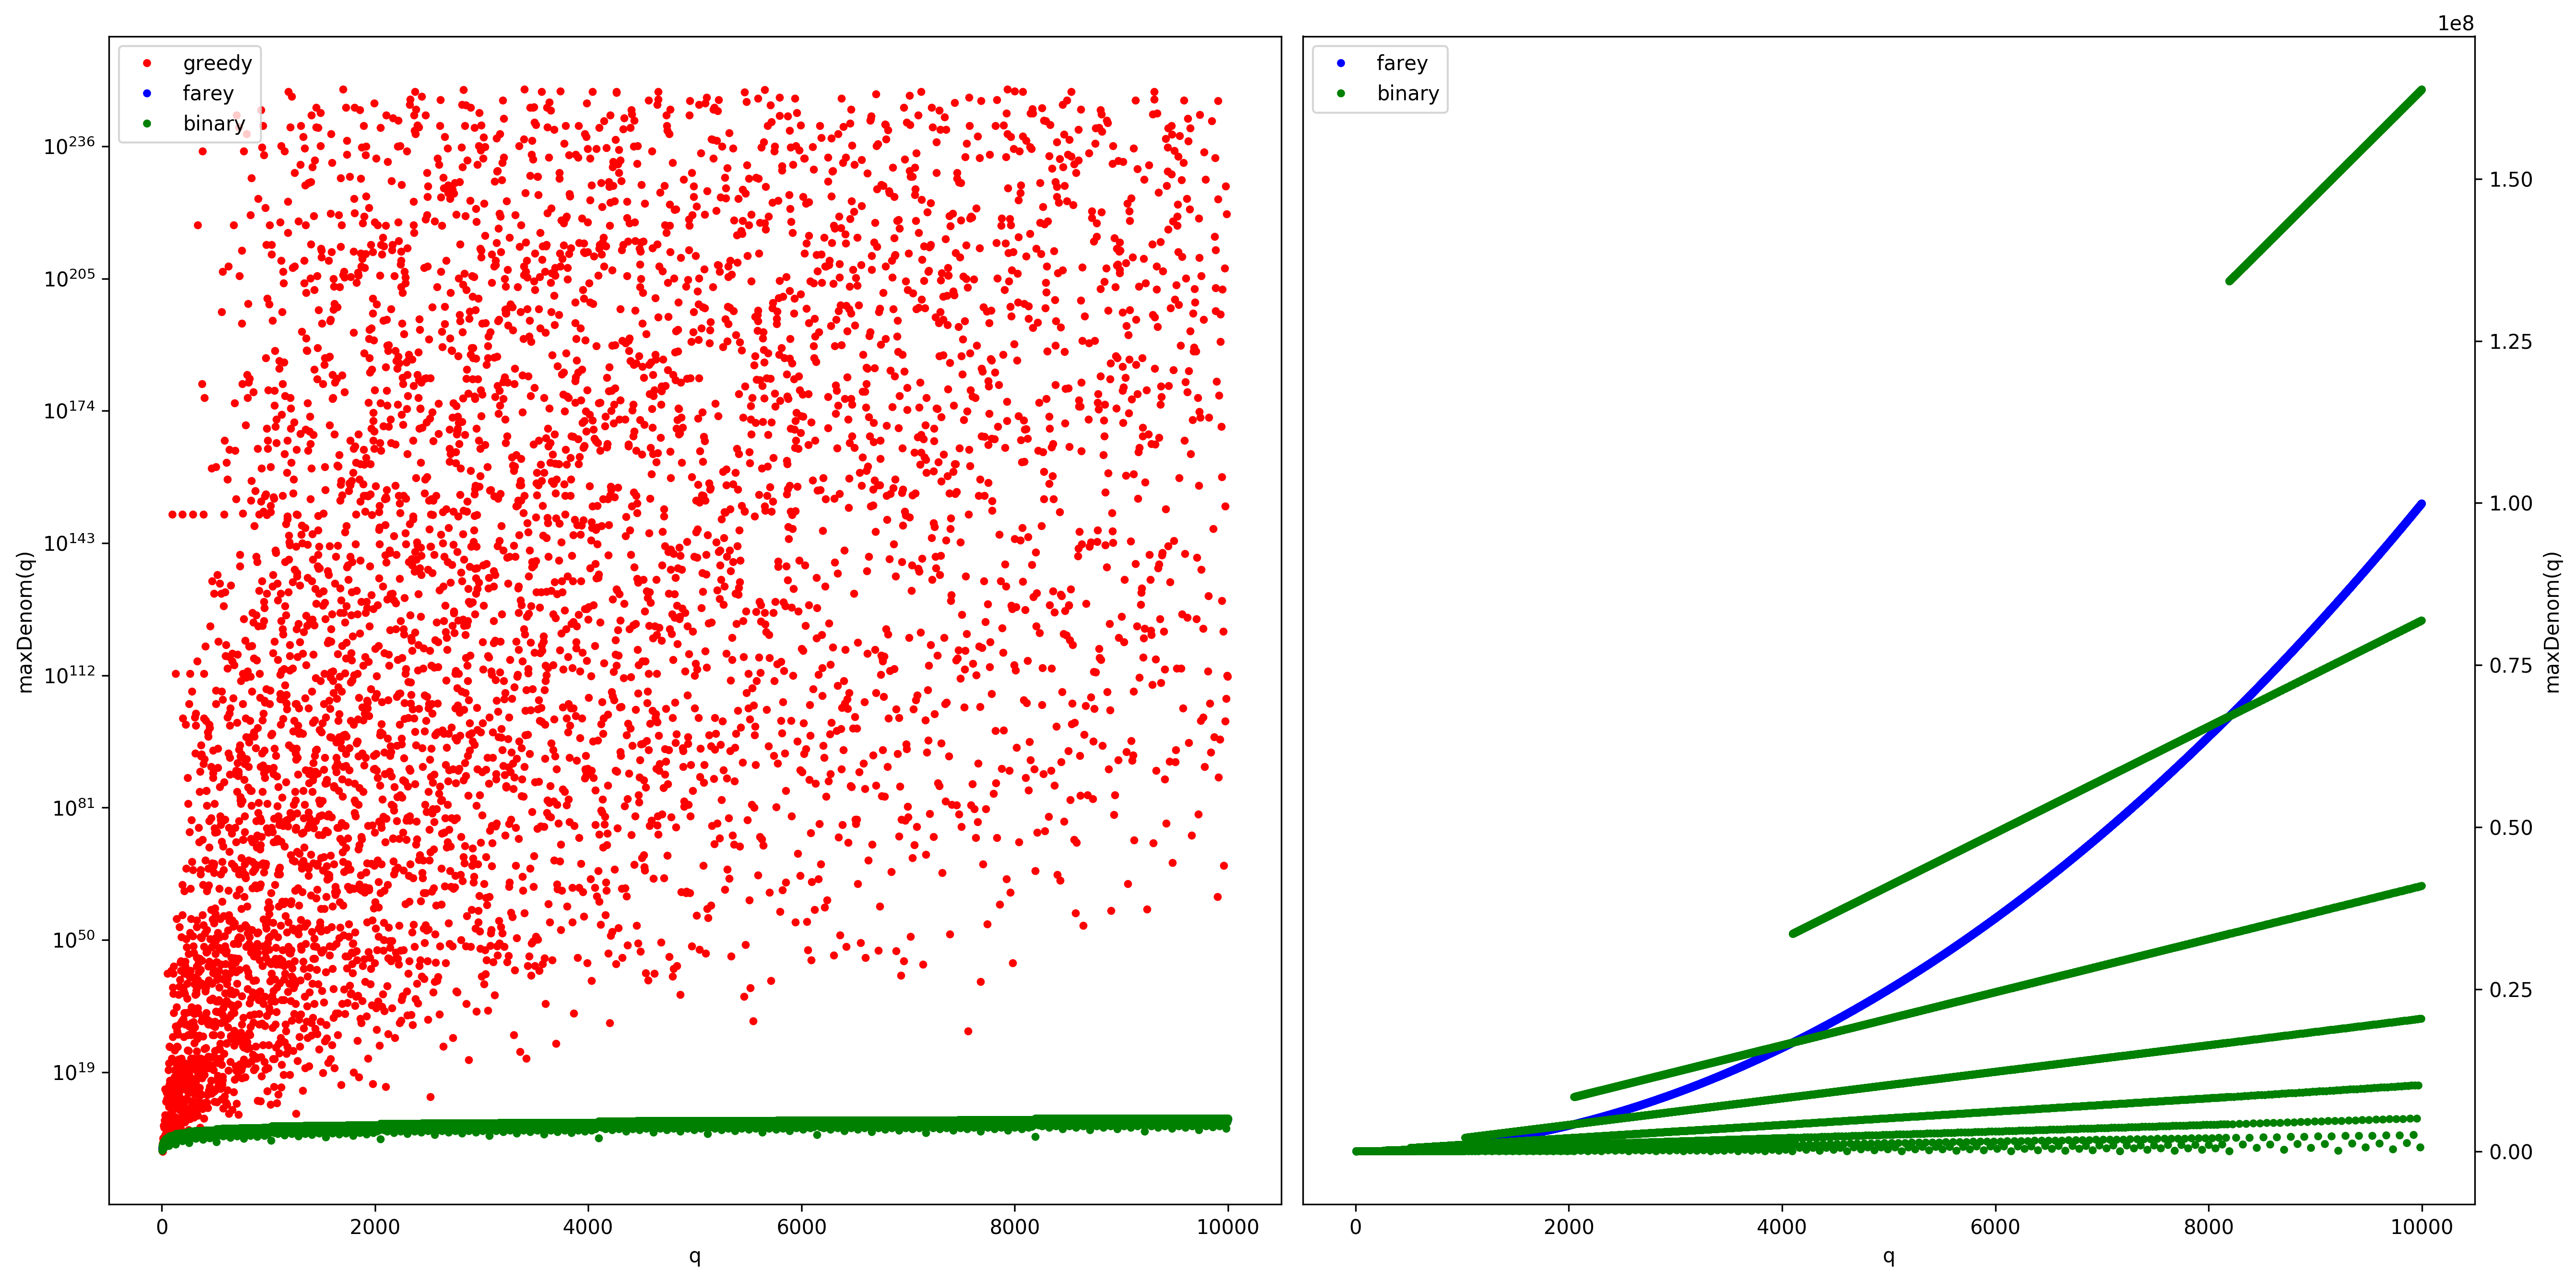
\includegraphics[width=\textwidth]{images/maxDenom2in1.png}
	\end{figure}
}{}

\subsubsection{Zusammenhang innerhalb des Binäralgorithmus}\label{subsubsec:ZsmHangBinary}
Im Binary-Algorithmus konnte eine einfache, aber aussagekräftige Korrelation zwischen $n$ und $minDenom(n)$ nachgewiesen werden:
\begin{equation*}
	minDenom_{binary}(n) = 
	\begin{cases}
		n & \text{falls n Zweierpotenz ist} \\
		2n & \text{sonst.}
	\end{cases}
\end{equation*}
Begründen lässt sich das mit der Zerlegung des Zählers im Schritt 2 des Algorithmus \ref{algo:binary}, für den bei ungeraden Nennern in der Zerlegung immer eine 1 vorkommt, die nicht mit dem Zähler $n$ gekürzt werden kann und somit den kleinsten Bruch $\uf{n}$ bildet. Falls der Zähler des zu zerlegenden Bruchs gerade ist, kann durch das Kürzen der Nenner nur kleiner werden. Für alle $n$, die Zweierpotenz sind, folgt $minDenom_{binary}(n) = n$. Für den Fall, dass n keine Zweierpotenz ist, entsteht der größte Nenner wieder durch den letzten Term in der Gleichung $\frac{p}{q} = .. = \frac{s}{N_k}+\frac{r}{qN_k}$ aus Schritt 3 des Algorithmus \ref{algo:binary}. Dabei ist in jedem Datensatz einmal das n derart gewählt, dass $\uf{2n} = \frac{r}{nN_k} \gdw r = \frac{N_k}{2}$ gilt. Dadurch ergibt sich der Term $\frac{r}{qN_k} = \uf{2q}$ und es entsteht der Zusammenhang $minDenom_{binary}(n) = 2n$ für alle n, die nicht Zweierpotenz sind.

\subsubsection{Vergleich mit Erwartungswerten}
Zur Überprüfung der in Tabelle \ref{table:Algo_Vergleich} aufgezeigten oberen Schranken sollen diese Werte mit den Ergebnissen der zuvor beschriebenen Testreihen verglichen werden.

\paragraph{Anzahl der Summanden}Die oberen Schranken für sowohl Greedy- als auch Farey-Folgen-Al\-go\-rith\-mus sind hier mit $p$, der Zähler des betrachteten Bruchs, angegeben, beim Binäralgorithmus ist hier nur die Komplexitätsklasse $O(\log q)$ angegeben. Bei Betrachtung der Ergebnisse, die in \ref{img:maxTerms} zusammengefasst sind, zeigen sich der Farey-Folgen- und der Binäralgorithmus mit genau dem erwarteten Verhalten, der Greedy-Algorithmus bleibt sogar weit unter seiner theoretischen Schranke und weist anstelle eines linearen Wachstums nur logarithmisches auf.
\paragraph{Größe der Nenner}Die größtmöglichen Nenner für den Binäralgorithmus werden mit $2(q^2-q)$, für den Farey-Folgen-Algorithmus mit $q(q-1)$, angegeben. Wie an Abbildung \ref{img:maxDenom} zu erkennen ist, halten sowohl Farey-Folgen- wie auch Binäralgorithmus ihre jeweiligen oberen Schranken ein.
Der Greedy-Algorithmus liefert, wie Bleicher und Erdös in ihrem Artikel ''Denominators of Egyptian Fractions''\footnote{engl.: Nenner Ägyptischer Brüche, \cite[S. 157]{BleicherErdoes1976}} schon berichteten, ein exponentielles Wachstum der Nenner, die aufgrund ihrer Größe in Abbildung \ref{img:maxDenom} teilweise nicht dargestellt werden konnten.

\subsection{Zusammenfassung}
Der Greedy-Algorithmus ist der wohl schlechteste der Algorithmen, obwohl er bezüglich der Anzahl der Terme die besten Ergebnisse liefert. Grund dafür ist die Wahl des jeweils größten Nenners, wodurch es zu den extremen numerischen Ausbrüchen der Nenner kommt, die eine effiziente Nutzung des Algorithmus mittels normaler Computersysteme unmöglich macht, da die Standards vieler Programmiersprachen solch große \bzw kleine Zahlen nicht unterstützen. Durch die großen Schwankungen zwischen den Werten des Greedy-Algorithmus ist dieser zudem sehr unvorhersehbar. Obwohl er in den meisten Fällen durchaus brauchbare Ergebnisse liefert, ist nicht vorhersagbar, wann dies nicht der Fall ist. Im Vergleich dazu tendiert der Farey-Folgen-Algorithmus eher dazu, kleinere Nenner zu erzeugen, benötigt dafür im Durchschnitt aber deutlich mehr Terme. Der Binäralgorithmus bewegt sich in den verglichenen Kriterien meist zwischen den Werten der anderen Algorithmen, aber immer zum geringeren tendierend, von wenigen Punkten der maximalen Nenner abgesehen, in denen er dem Farey-Folgen-Algorithmus leicht unterlegen ist. Zudem hatte er im Vergleich die beste Laufzeit und nach allem Anschein auch den stabilsten Gesamtverlauf. Damit ist diese Berechnungsmethode wohl die gewinnbringendste, da sie mit relativ wenig Aufwand durchaus brauchbare Zerlegungen gemeiner in Ägyptische Brüche erzeugt.